\documentclass[aspectratio=169]{beamer}

\usetheme{Berlin}

\usepackage[brazilian]{babel}
\usepackage[T1]{fontenc}
\usepackage[utf8]{inputenc}

\title{Algoritmo de Dijkstra}
\author{J Carlos Viana F}

\usepackage{minted}

\definecolor{bg}{rgb}{0.95,0.95,0.95}

\newmintedfile[ccode]{c}{
bgcolor=bg,
fontfamily=tt,
fontsize=\scriptsize,
linenos=true,
numberblanklines=true,
numbersep=12pt,
numbersep=5pt,
gobble=0,
frame=leftline,
framerule=0.4pt,
framesep=2mm,
funcnamehighlighting=true,
tabsize=4,
obeytabs=false,
mathescape=false
samepage=false, %with this setting you can force the list to appear on the same page
showspaces=false,
showtabs =false,
texcl=false,
}

\begin{document}

\frame{\titlepage}

\section{Dijkstra’s algorithm}

\begin{frame}
\cite[p. 658]{Cormen}
Dijkstra’s algorithm solves the single-source shortest-paths problem on a weighted,
directed graph G = (V,E) for the case in which all edge weights are nonnegative.
\end{frame}

\section{Pseudocódigo}

\begin{frame}
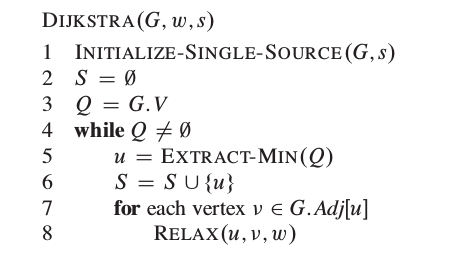
\includegraphics[scale=0.5]{cormen01.png}
\end{frame}

\begin{frame}
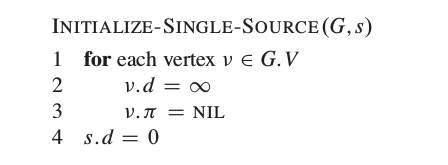
\includegraphics[scale=0.5]{cormen02.png}
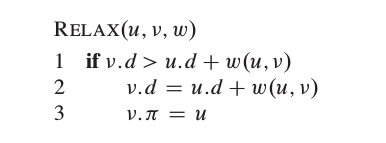
\includegraphics[scale=0.5]{cormen03.png}
\end{frame}

\section{Implementação}

\begin{frame}
\ccode[lastline=20]{code/dijkstra.c}
\end{frame}

\begin{frame}
\ccode[firstline=21,firstnumber=21,lastline=38]{code/dijkstra.c}
\end{frame}

\begin{frame}
\ccode[firstline=39,firstnumber=39,fontsize=\tiny]{code/dijkstra.c}
\end{frame}

\subsection{função extractMin}

\begin{frame}
\ccode{code/extractmin.c}
\end{frame}

\section{Referências}

\begin{frame}
\bibliographystyle{acm}
\bibliography{references}
\end{frame}

\end{document}
